\documentclass{article}
\usepackage{amsmath,amssymb,graphicx,enumitem,wrapfig}

\begin{document}
\parindent=0cm
\parskip=6pt
\pagestyle{empty}

%Begin
%Language English
%Source Cariboo College High School Mathematics competition
%Title Junior Preliminary Round 1973
%Question 1
%Subject arithmetic
%Category integers
%Type MC
%Choices 5
%Answer C
%Creator Victor Semenoff
%Rdifficulty 18
%Qtext

\scriptsize
Source: Cariboo College High School Mathematics Contest

\normalsize
%\begin{wrapfigure}[2]{r}[0pt]{0pt}
%	\includegraphics[width=30mm,viewport=]{CCJ78-04}
%\end{wrapfigure}
What is the smallest number which can be divided evenly by all of the following numbers: 3, 9, 12?\\
%ChoiceA
(A) 18\\
%ChoiceB
(B) 24\\
%ChoiceC
(C) 36\\
%ChoiceD
(D) 48\\
%ChoiceE
(E) 54\\
%Ftext

%\begin{wrapfigure}{r}[0pt]{0pt}
%	\includegraphics[width=30mm,viewport=]{CCJ78-04}
%\end{wrapfigure}

\textbf{The correct answer is (C): 36}\\[1 ex]
The smallest number that can be divided by 3, 9, and 12 is the lowest common multiple of these three numbers.  The prime factors of 3 are 3, of 9 are $3^2$ and of 12 are $2^2*3$.
Thus the lowest common multiple is $2*2*3*3=36$.
%End
\\[5 ex]
%Begin
%Language English
%Source Cariboo College High School Mathematics competition
%Title Junior Preliminary Round 1973
%Question 2
%Subject arithmetic
%Category fractions
%Type MC
%Choices 5
%Answer E
%Creator Victor Semenoff
%Rdifficulty 15
%Qtext

\scriptsize
Source: Cariboo College High School Mathematics Contest

\normalsize
%\begin{wrapfigure}[2]{r}[0pt]{0pt}
%	\includegraphics[width=30mm]{CCJ78-04}
%\end{wrapfigure}
$1/2$ of 90 is the same as $1/4$ of:\\
%ChoiceA
(A) 45\\
%ChoiceB
(B) 60\\
%ChoiceC
(C) 100\\
%ChoiceD
(D) 135\\
%ChoiceE
(E) 180\\
%Ftext

%\begin{wrapfigure}{r}[0pt]{0pt}
%	\includegraphics[width=30mm]{CCJ78-04}
%\end{wrapfigure}

\textbf{The correct answer is (E): 180}\\
We must find a number, $x$, such that $\frac{1}{2}\*90=\frac{1}{4}\*x$.  Multiplying both sides of the equation by 4, we find that $x=180$.
%End
\\[5 ex]
%Begin
%Language English
%Source Cariboo College High School Mathematics competition
%Title Junior Preliminary Round 1973
%Question 3
%Subject arithmetic
%Category integers
%Type MC
%Choices 5
%Answer B
%Creator Victor Semenoff
%Rdifficulty 14
%Qtext

\scriptsize
Source: Cariboo College High School Mathematics Contest

\normalsize
%\begin{wrapfigure}[2]{r}[0pt]{0pt}
%	\includegraphics[width=30mm]{CCJ78-04}
%\end{wrapfigure}
Which of the following multiples of 11 is also a multiple of 7?\\
%ChoiceA
(A) 1100\\
%ChoiceB
(B) 154\\
%ChoiceC
(C) 99\\
%ChoiceD
(D) 88\\
%ChoiceE
(E) 55\\
%Ftext

%\begin{wrapfigure}{r}[0pt]{0pt}
%	\includegraphics[width=30mm]{CCJ78-04}
%\end{wrapfigure}

\textbf{The correct answer is (B): 154}\\
Since 7 is prime, any number that is a multiple of 7 must have 7 to at least the $1^{st}$ power in its prime factorization. The prime factorizations of the numbers given are:\\
\begin{align*} 
1100 &=11\times10^2=11\times5^{2}\times2^2\\
154 &=11\times14=11\times7\times2\\
99 &=11\times9=11\times3^2\\
88 &=11\times8=11\times2^3\\
55 &=11\times5
\end{align*}
So 154 is the only multiple of 7.
%End
\\[5 ex]
%Begin
%Language English
%Source Cariboo College High School Mathematics competition
%Title Junior Preliminary Round 1973
%Question 4
%Subject arithmetic
%Category fractions
%Type MC
%Choices 5
%Answer A
%Creator Victor Semenoff
%Rdifficulty 13
%Qtext

\scriptsize
Source: Cariboo College High School Mathematics Contest

\normalsize
%\begin{wrapfigure}[2]{r}[0pt]{0pt}
%	\includegraphics[width=30mm]{CCJ78-04}
%\end{wrapfigure}
75\% of 360 is the same as:\\
%ChoiceA
(A) $3\times90$\\
%ChoiceB
(B) $300\times90$\\
%ChoiceC
(C) $75\times36$\\
%ChoiceD
(D) $.75\times36$\\
%ChoiceE
(E) None of the above\\
%Ftext

%\begin{wrapfigure}{r}[0pt]{0pt}
%	\includegraphics[width=30mm]{CCJ78-04}
%\end{wrapfigure}

\textbf{The correct answer is (A): $3\times90$}\\
Since 75\% of 360 is 270, and $270=3\times90$.
%End
\\[5 ex]
%Begin
%Language English
%Source Cariboo College High School Mathematics competition
%Title Junior Preliminary Round 1973
%Question 5
%Subject arithmetic
%Category integers
%Type MC
%Choices 5
%Answer B
%Creator Victor Semenoff
%Rdifficulty 13
%Qtext

\scriptsize
Source: Cariboo College High School Mathematics Contest

\normalsize
%\begin{wrapfigure}[2]{r}[0pt]{0pt}
%	\includegraphics[width=30mm]{CCJ78-04}
%\end{wrapfigure}
Which of the following is \textbf{not} evenly divisible by 6?\\
%ChoiceA
(A) 4284\\
%ChoiceB
(B) 2726\\
%ChoiceC
(C) 3426\\
%ChoiceD
(D) 8286\\
%ChoiceE
(E) 2244\\
%Ftext

%\begin{wrapfigure}{r}[0pt]{0pt}
%	\includegraphics[width=30mm]{CCJ78-04}
%\end{wrapfigure}

\textbf{The correct answer is (B): 2726}\\
Since $6=2\times3$, any number that is a multiple of 6 must also be a multiple of both 2 and 3.  Since all the numbers given are even, they are all multiples of 2.  We must check which numbers are multiples of 3.  If a number is a multiple of 3, the sum of its digits must be a multiple of 3.  Using this fact, we find that only 2726 is not a multiple of 3; thus 2726 is not evenly divisible by 6.
%End
\\[5 ex]
%Begin
%Language English
%Source Cariboo College High School Mathematics competition
%Title Junior Preliminary Round 1973
%Question 6
%Subject algebra
%Category concepts
%Type MC
%Choices 5
%Answer E
%Creator Victor Semenoff
%Rdifficulty 25
%Qtext

\scriptsize
Source: Cariboo College High School Mathematics Contest

\normalsize
%\begin{wrapfigure}[2]{r}[0pt]{0pt}
%	\includegraphics[width=30mm,viewport=]{CCJ78-04}
%\end{wrapfigure}
The following are numbers written in base 5. Which one is a prime number?\\
%ChoiceA
(A) 11\\
%ChoiceB
(B) 101\\
%ChoiceC
(C) 102\\
%ChoiceD
(D) 103\\
%ChoiceE
(E) 104\\
%Ftext

%\begin{wrapfigure}{r}[0pt]{0pt}
%	\includegraphics[width=30mm,viewport=]{CCJ78-04}
%\end{wrapfigure}
\textbf{The correct answer is (E): 104}\\
Let $[n]_{b}$ denote the number $n$ in base $b$. The numbers given in the question are then:
\begin{align*} 
[11]_{5} &=[1\times5^{1}+1\times5^{0}]_{10}=[5+1]_{10}=[6]_{10}\\
[101]_{5} &=[1\times5^{2}+1\times5^{0}]_{10}=[25+1]_{10}=[26]_{10}\\
[102]_{5} &=[101]_{5}+1=[27]_{10}\\
[103]_{5} &=[102]_{5}+1=[28]_{10}\\
[104]_{5} &=[103]_{5}+1=[29]_{10}
\end{align*}
Of the numbers listed, we see that only $[104]_{5}=[29]_{10}$ is prime.
%End
\\[5 ex]
%Begin
%Language English
%Source Cariboo College High School Mathematics competition
%Title Junior Preliminary Round 1973
%Question 7
%Subject geometry
%Category area
%Type MC
%Choices 5
%Answer C
%Creator Victor Semenoff
%Rdifficulty 17
%Qtext

\scriptsize
Source: Cariboo College High School Mathematics Contest

\normalsize
\begin{wrapfigure}[2]{r}[0pt]{0pt}
	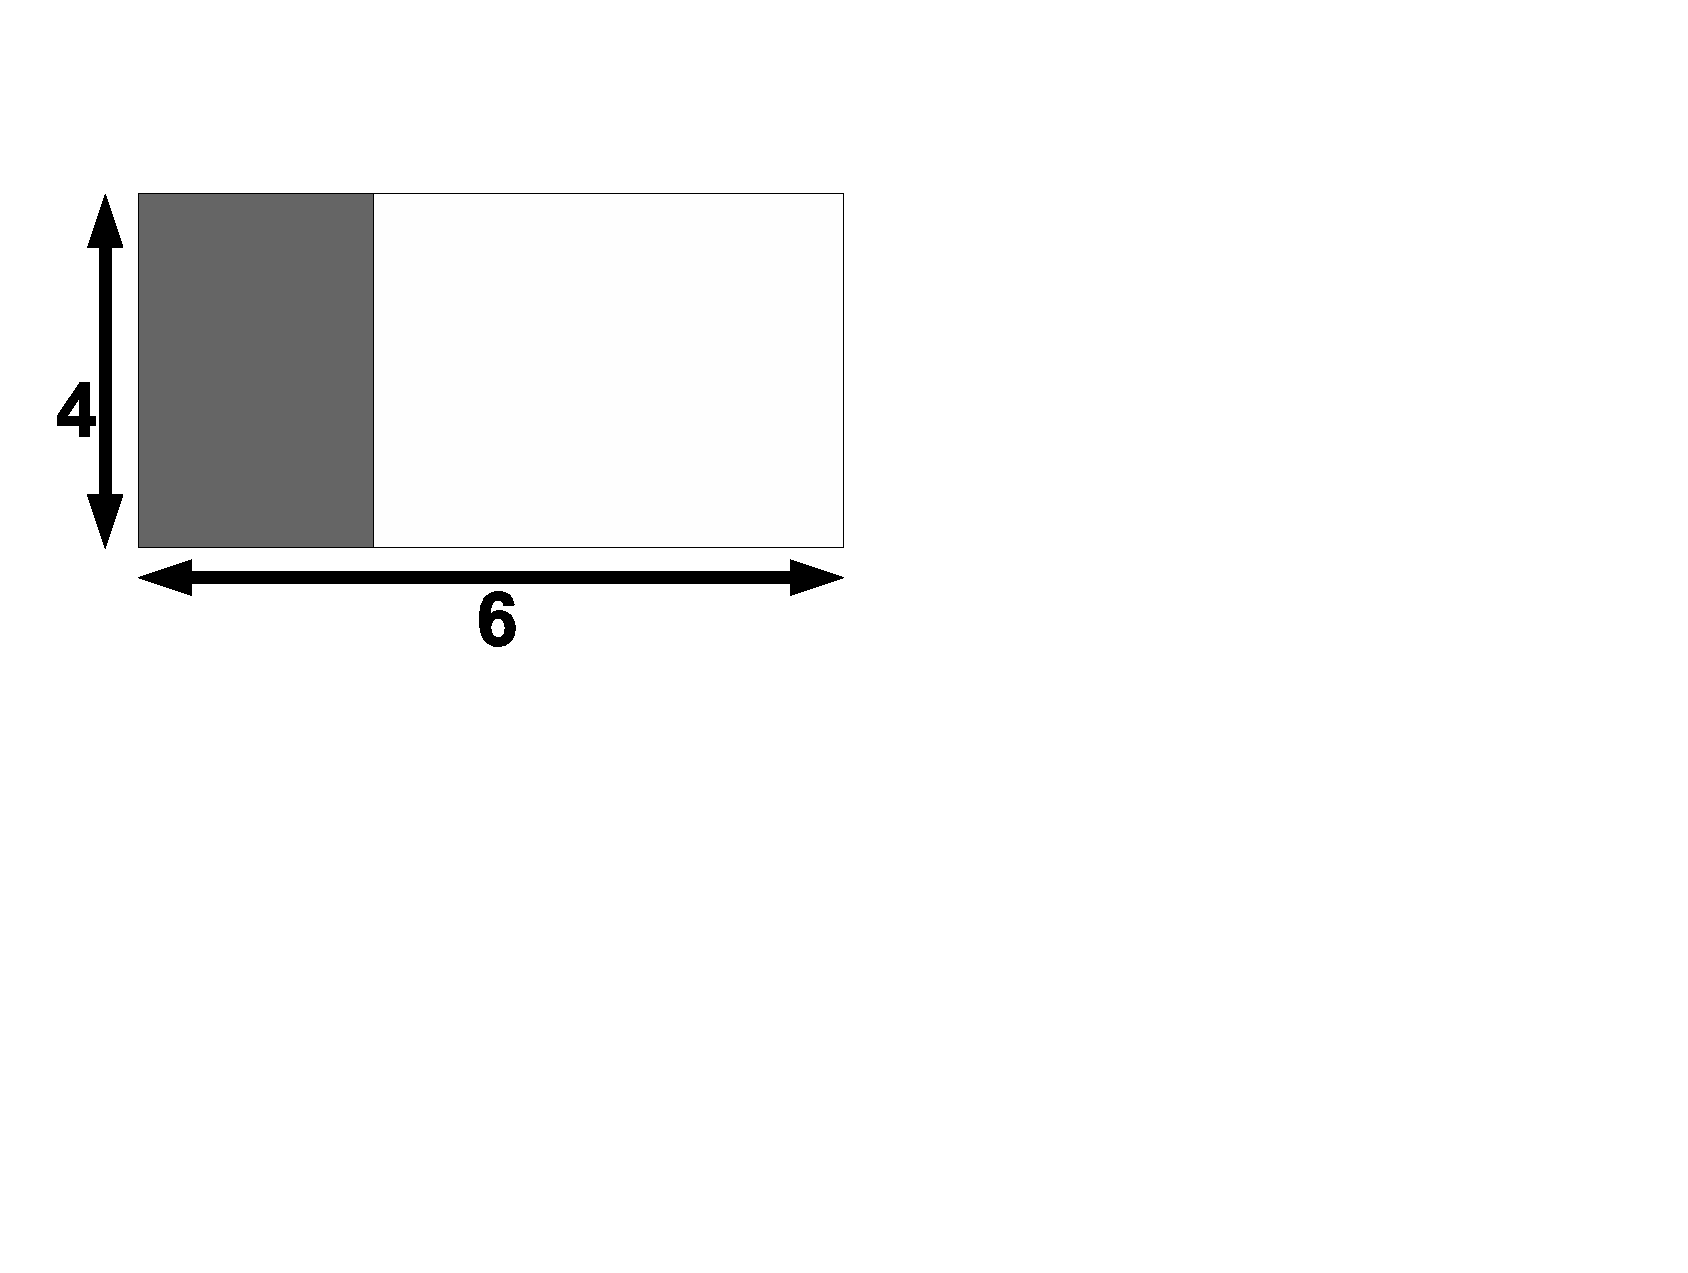
\includegraphics[width=30mm,viewport=17 290 402 516]{CCJPR73-7pic.eps}
\end{wrapfigure}
In the figure, if the length of the large rectangle is 6 and its width is 4, find the area of the small shaded rectangle if the remaining rectangle is a square.\\
%ChoiceA
(A) 24\\
%ChoiceB
(B) 12\\
%ChoiceC
(C) 8\\
%ChoiceD
(D) 6\\
%ChoiceE
(E) Not enough information\\
%Ftext

\begin{wrapfigure}{r}[0pt]{0pt}
	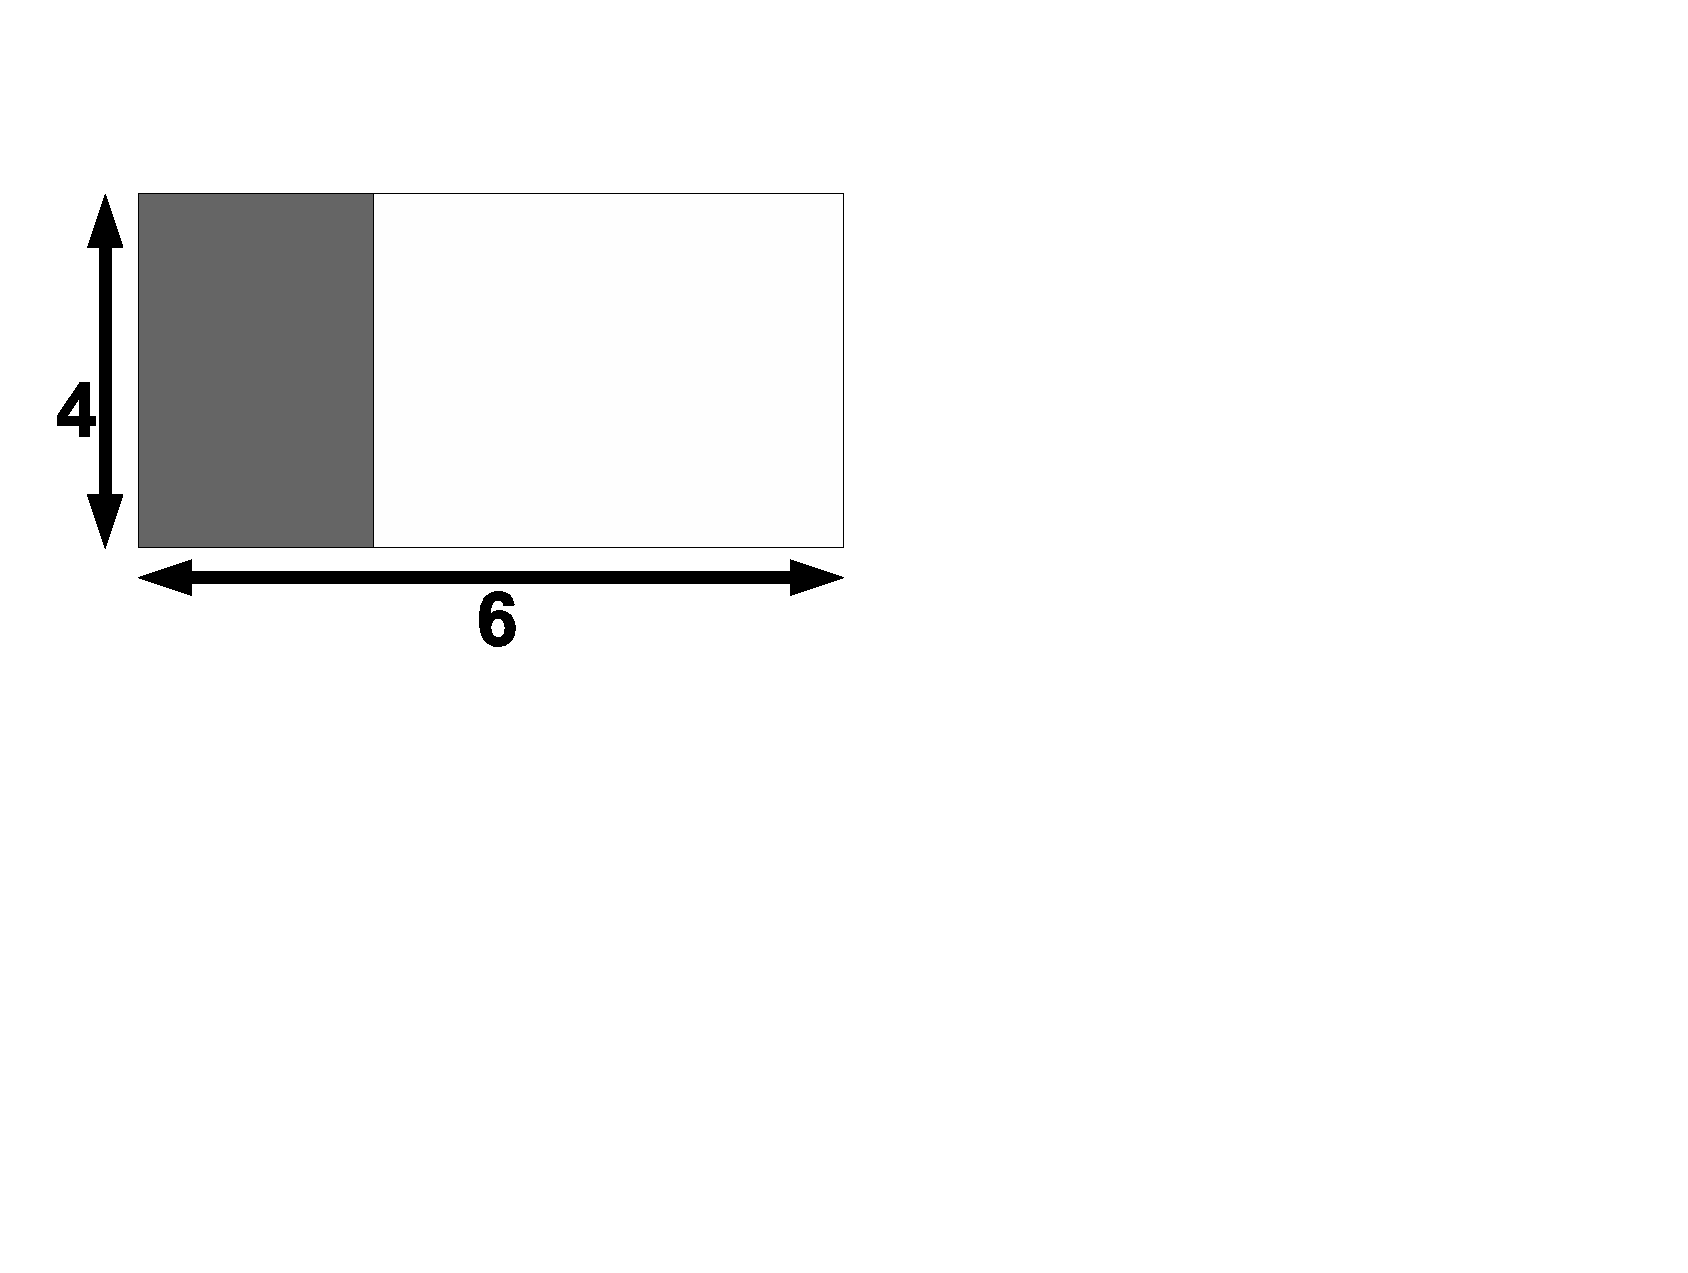
\includegraphics[width=30mm,viewport=17 290 402 516]{CCJPR73-7pic.eps}
\end{wrapfigure}

\textbf{The correct answer is (C): 8}\\[1ex]
The area of the large rectangle is equal to its length times its width: $4*6=24$.  The width of the square is equal to the width of the rectangle, or 4. Thus the area of the square is: $4*4=16$. The shaded region then has an area of $24-16=8$.
%End
\\[5 ex]
%Begin
%Language English
%Source Cariboo College High School Mathematics competition
%Title Junior Preliminary Round 1973
%Question 8
%Subject statistics
%Category concepts
%Type MC
%Choices 5
%Answer E
%Creator Victor Semenoff
%Rdifficulty 16
%Qtext

\scriptsize
Source: Cariboo College High School Mathematics Contest

\normalsize
%\begin{wrapfigure}[2]{r}[0pt]{0pt}
%	\includegraphics[width=30mm,viewport=]{CCJ78-04}
%\end{wrapfigure}
There are 30 students in a class. Twenty-four belong to the hiking club, and 13 are members of the chess club. Every member of the class belongs to at least one of these clubs. How many belong to both?\\
%ChoiceA
(A) 24\\
%ChoiceB
(B) 17\\
%ChoiceC
(C) 12\\
%ChoiceD
(D) 11\\
%ChoiceE
(E) 7\\
%Ftext

%\begin{wrapfigure}{r}[0pt]{0pt}
%	\includegraphics[width=30mm,viewport=]{CCJ78-04}
%\end{wrapfigure}

\textbf{The correct answer is (E): 7}\\[1 ex]
Let $b$ be the number of students who belong to both clubs. Suppose we were to count the number of students in each club and add them. We would then have counted each student who belonged to only one club once, and each student who belonged to both clubs twice. Thus adding would give $30+b$ total students.  Since we are told there are 24 members in the hiking club and 13 members in the chess club, we see that $30+b=37$.  Therefore, $b=7$.
%End
\\[5 ex]
%Begin
%Language English
%Source Cariboo College High School Mathematics competition
%Title Junior Preliminary Round 1973
%Question 9
%Subject statistics
%Category concepts
%Type MC
%Choices 5
%Answer E
%Creator Victor Semenoff
%Rdifficulty 18
%Qtext

\scriptsize
Source: Cariboo College High School Mathematics Contest

\normalsize
%\begin{wrapfigure}[2]{r}[0pt]{0pt}
%	\includegraphics[width=30mm,viewport=]{CCJ78-04}
%\end{wrapfigure}
A student has an average of 70 for three tests. What must she score on the next test to have an average of 75?\\
%ChoiceA
(A) 80\\
%ChoiceB
(B) 85\\
%ChoiceC
(C) 98\\
%ChoiceD
(D) 95\\
%ChoiceE
(E) 90\\
%Ftext

%\begin{wrapfigure}{r}[0pt]{0pt}
%	\includegraphics[width=30mm,viewport=]{CCJ78-04}
%\end{wrapfigure}

\textbf{The correct answer is (E): 90}\\[1 ex]
Let $S$ be the sum of the student's marks on the first 3 tests. Since her average mark on the tests was 70, $\frac{S}{3}=70$, meaning that $S=210$. For her average to be 75 after 4 tests, she must score a mark, $m$, such that $\frac{S+m}{4}=75$. Solving for $m$, we find that $m=4\times75-S=300-210=90$.
%End
\\[5 ex]
%Begin
%Language English
%Source Cariboo College High School Mathematics competition
%Title Junior Preliminary Round 1973
%Question 10
%Subject geometry
%Category triangles
%Type MC
%Choices 5
%Answer B
%Creator Victor Semenoff
%Rdifficulty 15
%Qtext

\scriptsize
Source: Cariboo College High School Mathematics Contest

\normalsize
\begin{wrapfigure}[2]{r}[0pt]{0pt}
	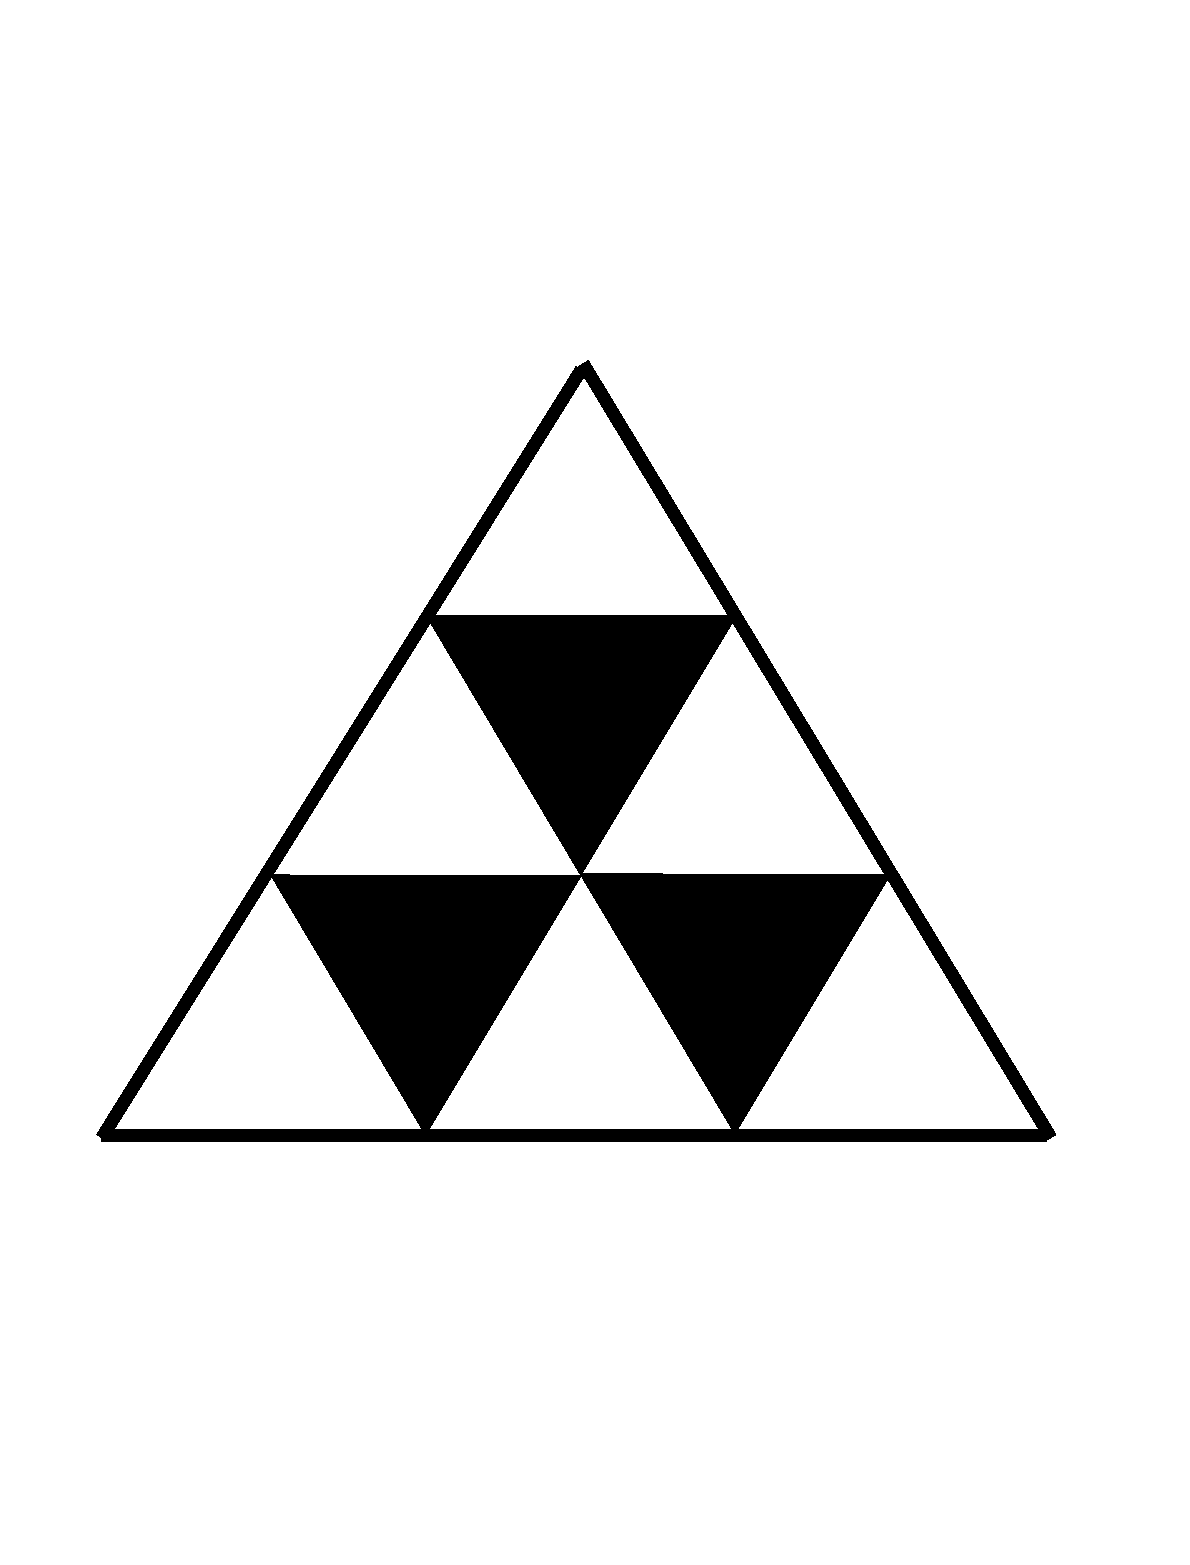
\includegraphics[width=30mm,viewport=33 187 502 584]{CCJPR73-10pic.eps}
\end{wrapfigure}
In the figure on the right, all the triangles appear to have the same area.  What percent of the figure is shaded?\\
%ChoiceA
(A) $66\frac{2}{3}$\\
%ChoiceB
(B) $33\frac{1}{3}$\\
%ChoiceC
(C) 40\\
%ChoiceD
(D) 50\\
%ChoiceE
(E) 25\\
%Ftext

\begin{wrapfigure}{r}[0pt]{0pt}
	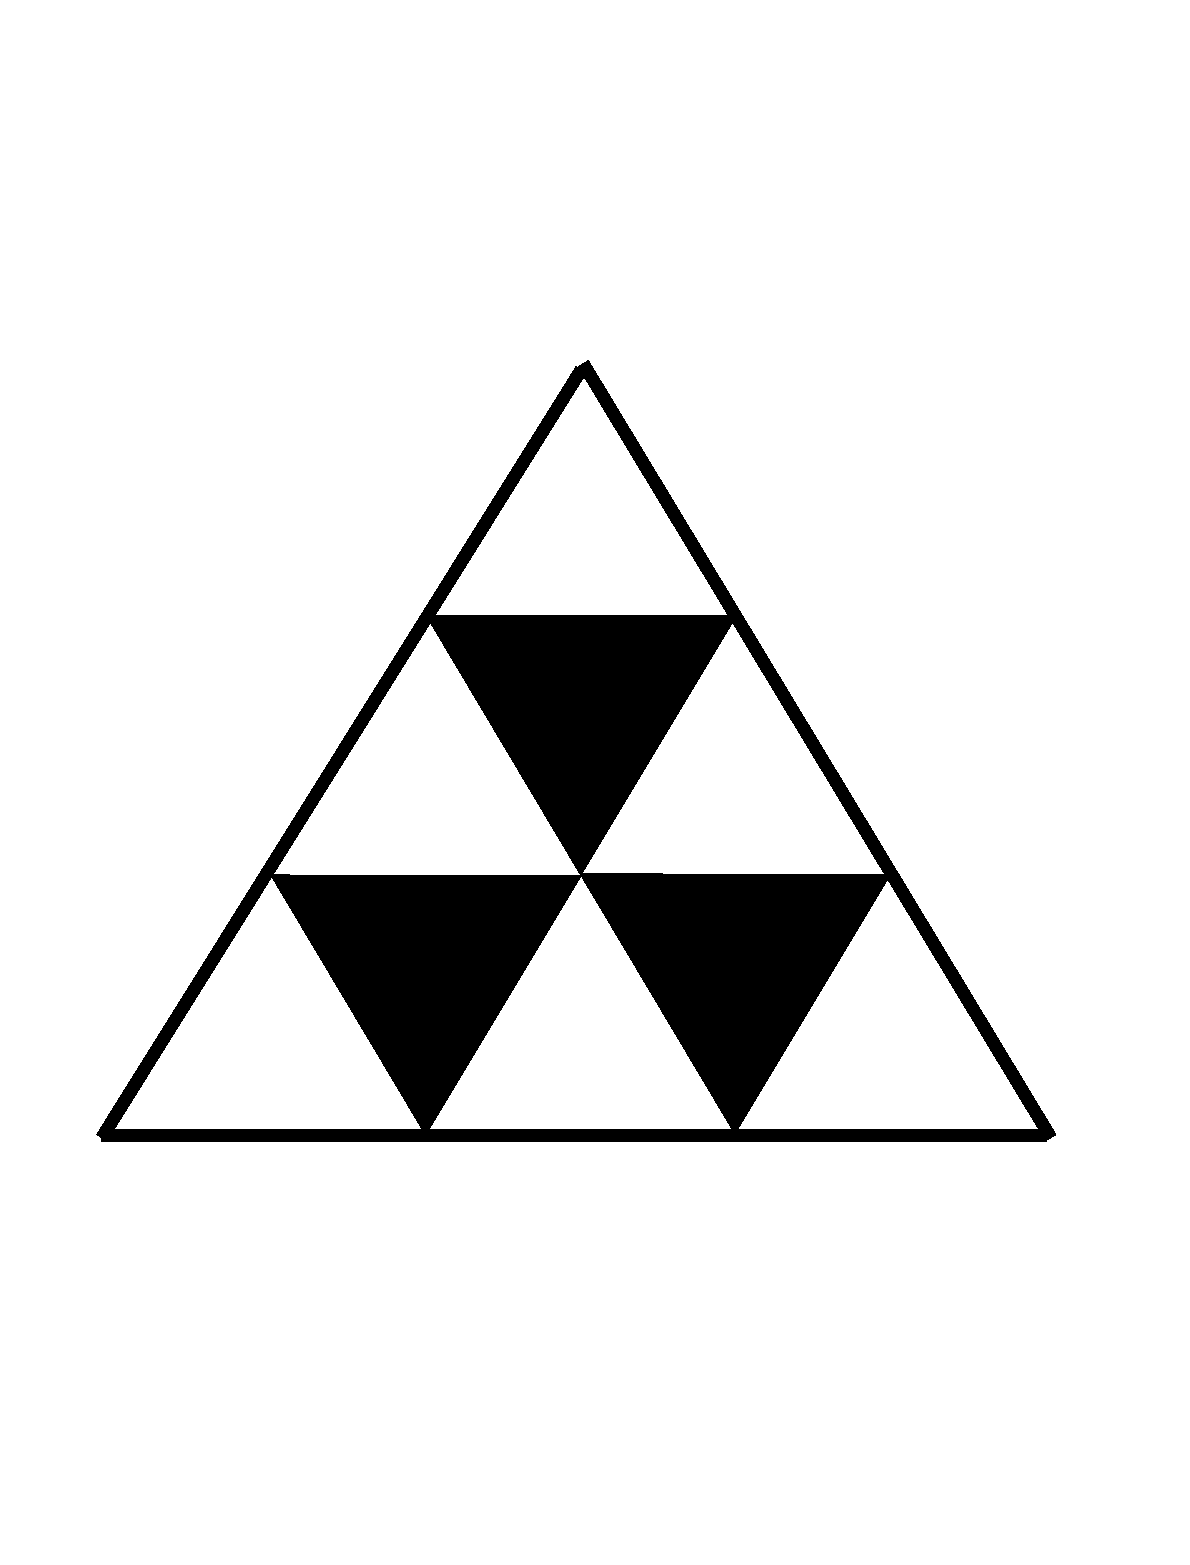
\includegraphics[width=30mm,viewport=33 187 502 584]{CCJPR73-10pic.eps}
\end{wrapfigure}

\textbf{The correct answer is (B): $33\frac{1}{3}$}\\[1 ex]
Let $a$ be the area of each of the smallest triangles in the figure. Since there are a total of 9 triangles, the total area of the figure will be $9a$.  Since 3 small triangles are shaded, the total area of the shaded region will be $3a$. Thus the percent of the figure that is shaded is
\begin{equation*}
\frac{\textrm{Shaded\space Area}}{\textrm{Total\space Area}}\times100\%=\frac{3a}{9a}\times100\%=\frac{1}{3}\times100\%=33\frac{1}{3}\%
\end{equation*}
%End
\\[5 ex]
%Begin
%Language English
%Source Cariboo College High School Mathematics competition
%Title Junior Preliminary Round 1973
%Question 11
%Subject arithmetic
%Category integers
%Type MC
%Choices 5
%Answer A
%Creator Victor Semenoff
%Rdifficulty 23
%Qtext

\scriptsize
Source: Cariboo College High School Mathematics Contest

\normalsize
%\begin{wrapfigure}[2]{r}[0pt]{0pt}
%	\includegraphics[width=30mm,viewport=]{CCJ78-04}
%\end{wrapfigure}
If the integer $n$ is divided by 8, the remainder is 3.  What will be the remainder when $5n$ is divided by 8?\\
%ChoiceA
(A) 7\\
%ChoiceB
(B) 6\\
%ChoiceC
(C) 5\\
%ChoiceD
(D) 3\\
%ChoiceE
(E) 1\\
%Ftext

%\begin{wrapfigure}{r}[0pt]{0pt}
%	\includegraphics[width=30mm,viewport=]{CCJ78-04}
%\end{wrapfigure}

\textbf{The correct answer is (A): 7}\\[1 ex]
Let $q$ be the quotient when $n$ is divided by 8. We can then write $n$ as $n=q+\frac{3}{8}$. Multiplying this equation by 5 gives:
\begin{equation*}
5n=5q+\frac{5\times3}{8}=5q+\frac{15}{8}= (5q+1)+\frac{7}{8}
\end{equation*}
From this we see that the remainder when $5n$ is divided by 8 is 7.
%End
\\[5 ex]
%Begin
%Language English
%Source Cariboo College High School Mathematics competition
%Title Junior Preliminary Round 1973
%Question 12
%Subject arithmetic
%Category integers
%Type MC
%Choices 5
%Answer B
%Creator Victor Semenoff
%Rdifficulty 15
%Qtext

\scriptsize
Source: Cariboo College High School Mathematics Contest

\normalsize
%\begin{wrapfigure}[2]{r}[0pt]{0pt}
%	\includegraphics[width=30mm,viewport=]{CCJ78-04}
%\end{wrapfigure}
When the sum of thirty numbers is doubled the result is 456,928. If one of the thirty numbers is changed from 18,425 to 16,425, what will be the result when the new sum is doubled?\\
%ChoiceA
(A) 454,928\\
%ChoiceB
(B) 452,928\\
%ChoiceC
(C) 434,928\\
%ChoiceD
(D) 453,928\\
%ChoiceE
(E) none of these\\
%Ftext

%\begin{wrapfigure}{r}[0pt]{0pt}
%	\includegraphics[width=30mm,viewport=]{CCJ78-04}
%\end{wrapfigure}

\textbf{The correct answer is (B): 452,928}\\[1 ex]
Let $S$ be the sum of the 30 numbers. Since twice the sum of these 30 numbers is 456,928, we have $2S=456,928$. When one of the numbers is changed from 18,425 to 16,425, the new sum, $S_{n}$, will be $S_{n}=S-18,425+16,425=S-2000$. Twice this new sum gives:
\begin{equation*}
2S_{n}=2(S-2000)=2S-4000=456,928-4000=452,928.
\end{equation*}
%End
\\[5 ex]
%Begin
%Language English
%Source Cariboo College High School Mathematics competition
%Title Junior Preliminary Round 1973
%Question 13
%Subject geometry
%Category area
%Type MC
%Choices 5
%Answer B
%Creator Victor Semenoff
%Rdifficulty 14
%Qtext

\scriptsize
Source: Cariboo College High School Mathematics Contest

\normalsize
%\begin{wrapfigure}[2]{r}[0pt]{0pt}
%	\includegraphics[width=30mm,viewport=]{CCJ78-04}
%\end{wrapfigure}
If $\frac{9}{16}$ of the area of a square is 4, what is the side length of the square?\\
%ChoiceA
(A) $\frac{8}{9}$\\[1 ex]
%ChoiceB
(B) $2\frac{2}{3}$\\[1 ex]
%ChoiceC
(C) $3\frac{1}{3}$\\[1 ex]
%ChoiceD
(D) $5\frac{1}{3}$\\[1 ex]
%ChoiceE
(E) $11\frac{1}{9}$\\
%Ftext

%\begin{wrapfigure}{r}[0pt]{0pt}
%	\includegraphics[width=30mm,viewport=]{CCJ78-04}
%\end{wrapfigure}

\textbf{The correct answer is (B): $2\frac{2}{3}$}\\[1 ex]
Let $l$ be the length of a side of the square. The area of the square will then be $l^{2}$. Since we are told $\frac{9}{16}$ of the area of the square is 4, we have:
\begin{align*}
\frac{9}{16}l^{2} &=4\\
l^{2} &=\frac{64}{9}\\
l &=\frac{8}{3}=2\frac{2}{3}
\end{align*}
%End
\\[5 ex]
%Begin
%Language English
%Source Cariboo College High School Mathematics competition
%Title Junior Preliminary Round 1973
%Question 14
%Subject arithmetic
%Category integers
%Type MC
%Choices 5
%Answer B
%Creator Victor Semenoff
%Rdifficulty 18
%Qtext

\scriptsize
Source: Cariboo College High School Mathematics Contest

\normalsize
%\begin{wrapfigure}[2]{r}[0pt]{0pt}
%	\includegraphics[width=30mm,viewport=]{CCJ78-04}
%\end{wrapfigure}
Two whole numbers are each bigger than one and their product is an odd number. The sum of the two numbers is:\\
%ChoiceA
(A) an even number greater than their product\\
%ChoiceB
(B) an even number less than their product\\
%ChoiceC
(C) an odd number greater than their product\\
%ChoiceD
(D) an odd number less than their product\\
%ChoiceE
(E) not enough information given\\
%Ftext

%\begin{wrapfigure}{r}[0pt]{0pt}
%	\includegraphics[width=30mm,viewport=]{CCJ78-04}
%\end{wrapfigure}

\textbf{The correct answer is (B): an even number less than their product}\\[1 ex]
Let $a$ and $b$ be the two numbers in question. Since their product is odd, both $a$ and $b$ are odd, and thus $a+b$ is \textbf{even}. Further, if we \textbf{assume} $a+b\geq ab$, then by dividing both sides by $ab$ we get :
\begin{equation*}
\frac{1}{a}+\frac{1}{b}\geq 1
\end{equation*}
The left side of this equation is a maximum when $a$ and $b$ are minima.  Since $a$ and $b$ are odd and greater than 1, the smallest they can be is 3.  Thus the largest the left side of the equation can be is $\frac{1}{3}+\frac{1}{3}=\frac{2}{3}$. And thus we know that
\begin{equation*}
Max(\frac{1}{a}+\frac{1}{b})=\frac{2}{3}\leq 1
\end{equation*}
But this violates our assumption $\frac{1}{a}+\frac{1}{b}\geq 1$, and thus our \textbf{assumption} is wrong.  Thus \begin{equation*}
\frac{1}{a}+\frac{1}{b}\leq 1
\end{equation*}
And thus we know that for $a$ and $b$, their sum is an even number less than their product.
%End
\\[5 ex]
%Begin
%Language English
%Source Cariboo College High School Mathematics competition
%Title Junior Preliminary Round 1973
%Question 15
%Subject functions
%Category absval
%Type MC
%Choices 5
%Answer C
%Creator Victor Semenoff
%Rdifficulty 19
%Qtext

\scriptsize
Source: Cariboo College High School Mathematics Contest

\normalsize
%\begin{wrapfigure}[2]{r}[0pt]{0pt}
%	\includegraphics[width=30mm,viewport=]{CCJ78-04}
%\end{wrapfigure}
Given three integers $a$, $b$, and $c$ such that $a<b<c<0$, which one of the following statements is true?\\
%ChoiceA
(A) $a>c$\\
%ChoiceB
(B) $ab<bc$\\
%ChoiceC
(C) $ab>0$\\
%ChoiceD
(D) $bc<0$\\
%ChoiceE
(E) $c-b<0$\\
%Ftext

%\begin{wrapfigure}{r}[0pt]{0pt}
%	\includegraphics[width=30mm,viewport=]{CCJ78-04}
%\end{wrapfigure}

\textbf{The correct answer is (C): $ab>0$}\\[1 ex]
Since $a$ and $b$ are both negative, we know that $ab>0$. It is easy to verify that none of the other choices are true.
%End
\\[5 ex]
%Begin
%Language English
%Source Cariboo College High School Mathematics competition
%Title Junior Preliminary Round 1973
%Question 16
%Subject arithmetic
%Category fractions
%Type MC
%Choices 5
%Answer C
%Creator Victor Semenoff
%Rdifficulty 20
%Qtext

\scriptsize
Source: Cariboo College High School Mathematics Contest

\normalsize
%\begin{wrapfigure}[2]{r}[0pt]{0pt}
%	\includegraphics[width=30mm,viewport=]{CCJ78-04}
%\end{wrapfigure}
What is the largest integer $n$ for which $\frac{4}{3}n<\frac{34}{5}$?\\
%ChoiceA
(A) 8\\
%ChoiceB
(B) 6\\
%ChoiceC
(C) 5\\
%ChoiceD
(D) 3\\
%ChoiceE
(E) 0\\
%Ftext

%\begin{wrapfigure}{r}[0pt]{0pt}
%	\includegraphics[width=30mm,viewport=]{CCJ78-04}
%\end{wrapfigure}

\textbf{The correct answer is (C): 5}\\[1 ex]
Let $\frac{4n}{3}<\frac{34}{5}$, then we have:\\
\begin{equation*}
n<\frac{34}{5}\times\frac{3}{4}=\frac{51}{10}=5.1
\end{equation*}
Thus the largest integer that satisfies the inequality is 5.
%End
\\[5 ex]
%Begin
%Language English
%Source Cariboo College High School Mathematics competition
%Title Junior Preliminary Round 1973
%Question 17
%Subject logic
%Category general
%Type MC
%Choices 5
%Answer D
%Creator Victor Semenoff
%Rdifficulty 15
%Qtext

\scriptsize
Source: Cariboo College High School Mathematics Contest

\normalsize
%\begin{wrapfigure}[2]{r}[0pt]{0pt}
%	\includegraphics[width=30mm,viewport=]{CCJ78-04}
%\end{wrapfigure}
Given the two statements:
\begin{enumerate}
\item{At least one Pooh is a Winnie.}
\item{No Winnies are bears.}
\end{enumerate} 
are true, we may conclude that:\\
%ChoiceA
(A) At least one Pooh is not a Winnie.\\
%ChoiceB
(B) No Poohs are bears.\\
%ChoiceC
(C) At least one Pooh is a bear.\\
%ChoiceD
(D) At least one Pooh is not a bear.\\
%ChoiceE
(E) None of A, B, C, or D may be concluded.\\
%Ftext

%\begin{wrapfigure}{r}[0pt]{0pt}
%	\includegraphics[width=30mm,viewport=]{CCJ78-04}
%\end{wrapfigure}

\textbf{The correct answer is (D): At least one Pooh is not a bear.\\}\\[1 ex]
Let $P$ be one of the Poohs that is a Winnie (from statement 1 we know that there is at least one). Since $P$ is a Winnie, and (by statement 2) no Winnies are bears, $P$ is not a bear.  Thus there is at least one Pooh that is not a bear.
%End
\\[5 ex]
%Begin
%Language English
%Source Cariboo College High School Mathematics competition
%Title Junior Preliminary Round 1973
%Question 18
%Subject geometry
%Category length
%Type MC
%Choices 5
%Answer A
%Creator Victor Semenoff
%Rdifficulty 25
%Qtext

\scriptsize
Source: Cariboo College High School Mathematics Contest

\normalsize
%\begin{wrapfigure}[2]{r}[0pt]{0pt}
%	\includegraphics[width=30mm,viewport=]{CCJ78-04}
%\end{wrapfigure}
A board 82 inches long is to be cut into four lengths so that the first piece is twice the length of the second piece, which is three times the length of the third piece, which is four times the length of the fourth piece. Find the length of the longest piece in inches.\\
%ChoiceA
(A) 48\\
%ChoiceB
(B) $32\frac{4}{5}$\\
%ChoiceC
(C) 24\\
%ChoiceD
(D) $8\frac{1}{5}$\\
%ChoiceE
(E) 2\\
%Ftext

%\begin{wrapfigure}{r}[0pt]{0pt}
%	\includegraphics[width=30mm,viewport=]{CCJ78-04}
%\end{wrapfigure}

\textbf{The correct answer is (A): 48}\\[1 ex]
Let $l_{n}$ be the length of the $n^{\mathrm {th}}$ piece in inches. From the question we know that $l_1=2l_2$, $l_2=3l_3$, and $l_3=4l_4$.  We also know that $l_{1}+l_{2}+l_{3}+l_{4}=82$.  Thus we have four linear equations and the four unknowns $l_1$, $l_2$, $l_3$, and $l_4$.

Solving these gives:
\begin{align*}
l_{4}&=2\\
l_{3}&=8\\
l_{2}&=24\\
l_{1}&=48
\end{align*}
Thus the longest piece is 48 inches long.
%End
\\[5 ex]
%Begin
%Language English
%Source Cariboo College High School Mathematics competition
%Title Junior Preliminary Round 1973
%Question 19
%Subject algebra
%Category modelling
%Type MC
%Choices 5
%Answer C
%Creator Victor Semenoff
%Rdifficulty 23
%Qtext

\scriptsize
Source: Cariboo College High School Mathematics Contest

\normalsize
%\begin{wrapfigure}[2]{r}[0pt]{0pt}
%	\includegraphics[width=30mm,viewport=]{CCJ78-04}
%\end{wrapfigure}
Three gallons of wine are mixed with 5 gallons of water in a barrel.  If two gallons of the mixture are drawn off and a further 1 gallon of wine added to the remainder, how many gallons of water does the new mixture contain?\\
%ChoiceA
(A) 5\\[1 ex]
%ChoiceB
(B) $4\frac{1}{5}$\\[1 ex]
%ChoiceC
(C) $3\frac{3}{4}$\\[1 ex]
%ChoiceD
(D) $4\frac{1}{4}$\\[1 ex]
%ChoiceE
(E) $3\frac{1}{4}$\\
%Ftext

%\begin{wrapfigure}{r}[0pt]{0pt}
%	\includegraphics[width=30mm,viewport=]{CCJ78-04}
%\end{wrapfigure}

\textbf{The correct answer is (C): $3\frac{3}{4}$\\[1 ex]}\\[1 ex]
The initial mixture contains 3 gallons of wine, and 5 gallons of water for a total of 8 gallons.  Since $\frac{5}{8}$ of this mixture is water, when 2 gallons of the mixture are drawn off, $\frac{2\times5}{8}=\frac{5}{4}$ of a gallon of water will be lost, leaving a total of $5-\frac{5}{4}=3\frac{3}{4}$ gallons of water.  Adding wine will not affect the number of gallons of water in the mixture, meaning that the final mixture will contain $3\frac{3}{4}$ gallons of water.
%End
\\[5 ex]
%Begin
%Language English
%Source Cariboo College High School Mathematics competition
%Title Junior Preliminary Round 1973
%Question 20
%Subject algebra
%Category modelling
%Type MC
%Choices 5
%Answer D
%Creator Victor Semenoff
%Rdifficulty 25
%Qtext

\scriptsize
Source: Cariboo College High School Mathematics Contest

\normalsize
%\begin{wrapfigure}[2]{r}[0pt]{0pt}
%	\includegraphics[width=30mm,viewport=]{CCJ78-04}
%\end{wrapfigure}
A horse can run $1\frac{1}{4}$ miles in the same time as a man can run $\frac{1}{4}$ mile. If the horse and the man both start from the same place on a circular track of length $1\frac{1}{2}$ miles, what is the least number of circuits the horse must run before both horse and man arrive simultaneously back at the starting point?\\
%ChoiceA
(A) 2\\
%ChoiceB
(B) 3\\
%ChoiceC
(C) 4\\
%ChoiceD
(D) 5\\
%ChoiceE
(E) They will never arrive at the starting point together.\\
%Ftext

%\begin{wrapfigure}{r}[0pt]{0pt}
%	\includegraphics[width=30mm,viewport=]{CCJ78-04}
%\end{wrapfigure}

\textbf{The correct answer is (D): 5}\\[1 ex]
Since the horse can run $1\frac{1}{4}=\frac{5}{4}$ miles in the same time the man can run $\frac{1}{2}$ mile, the ratio of their speeds is
\begin{equation*}
\frac{5}{4}:\frac{1}{2}=5:2.
\end{equation*}
This means that the horse completes his fifth lap when the man completes his second.  Because 2 and 5 have no common factors, these are the fewest number of laps before they are back at the starting line together.
%End
\\[5 ex]
%Begin
%Language English
%Source Cariboo College High School Mathematics competition
%Title Junior Preliminary Round 1973
%Question 21
%Subject geometry
%Category 3D
%Type MC
%Choices 5
%Answer D
%Creator Victor Semenoff
%Rdifficulty 23
%Qtext

\scriptsize
Source: Cariboo College High School Mathematics Contest

\normalsize
%\begin{wrapfigure}[2]{r}[0pt]{0pt}
%	\includegraphics[width=30mm,viewport=]{CCJ78-04}
%\end{wrapfigure}
What is the ratio of the total volume of 3 spheres each 2 cm in diameter to the volume of 1 sphere 3 cm in diameter? (The volume of a sphere is given by the formula $V=\frac{4}{3}\pi r^3$, where $\pi\approx 3.14$.)\\
%ChoiceA
(A) 2:3\\
%ChoiceB
(B) 2:1\\
%ChoiceC
(C) 4:9\\
%ChoiceD
(D) 8:9\\
%ChoiceE
(E) none of these\\
%Ftext

%\begin{wrapfigure}{r}[0pt]{0pt}
%	\includegraphics[width=30mm,viewport=]{CCJ78-04}
%\end{wrapfigure}

\textbf{The correct answer is (D): 8:9}\\[1 ex]
Since the volume in $\mathrm{cm}^3$ of each of the 2 cm diameter spheres is $\frac{4}{3}\pi$, the total volume of all three is $3\times\frac{4}{3}\pi=4\pi$.
The volume of the 3 cm diameter sphere is $\frac{4}{3}\pi(\frac{2}{3})^3$. Thus the ratio of the volume of the three smaller spheres to the volume of the single larger sphere is
\begin{equation*}
3\times\frac{4}{3}\pi:\frac{4}{3}\pi(\frac{3}{2})^3=3:(\frac{3}{2})^3=3:\frac{27}{8}=8:9
\end{equation*}
%End
\\[5 ex]
%Begin
%Language English
%Source Cariboo College High School Mathematics competition
%Title Junior Preliminary Round 1973
%Question 22
%Subject arithmetic
%Category integers
%Type MC
%Choices 5
%Answer E
%Creator Victor Semenoff
%Rdifficulty 15
%Qtext

\scriptsize
Source: Cariboo College High School Mathematics Contest

\normalsize
%\begin{wrapfigure}[2]{r}[0pt]{0pt}
%	\includegraphics[width=30mm,viewport=]{CCJ78-04}
%\end{wrapfigure}
In a certain chess tournament a player is eliminated if he loses a game. If there were 24 contestants and no game ended in a draw, the number of games played to determine the final winner was:\\
%ChoiceA
(A) 276\\
%ChoiceB
(B) 48\\
%ChoiceC
(C) 47\\
%ChoiceD
(D) 24\\
%ChoiceE
(E) 23\\
%Ftext

%\begin{wrapfigure}{r}[0pt]{0pt}
%	\includegraphics[width=30mm,viewport=]{CCJ78-04}
%\end{wrapfigure}

\textbf{The correct answer is (E): 23}\\[1 ex]
Each game played eliminates one player. Since we need to eliminate 23 players, 23 games are needed to be played.
%End
\\[5 ex]
%Begin
%Language English
%Source Cariboo College High School Mathematics competition
%Title Junior Preliminary Round 1973
%Question 23
%Subject algebra
%Category modelling
%Type MC
%Choices 5
%Answer A
%Creator Victor Semenoff
%Rdifficulty 27
%Qtext

\scriptsize
Source: Cariboo College High School Mathematics Contest

\normalsize
%\begin{wrapfigure}[2]{r}[0pt]{0pt}
%	\includegraphics[width=30mm,viewport=]{CCJ78-04}
%\end{wrapfigure}
A cougar chases a deer. The cougar takes two leaps while the deer takes three. Each leap that the cougar takes covers as much ground as two of the deer's leaps. If, at the beginning of the chase, the deer was 20 of its leaps ahead of the cougar, how many leaps will the deer take before the cougar catches it?\\
%ChoiceA
(A) 60\\
%ChoiceB
(B) 40\\
%ChoiceC
(C) 20\\
%ChoiceD
(D) 17\\
%ChoiceE
(E) 10\\
%Ftext

%\begin{wrapfigure}{r}[0pt]{0pt}
%	\includegraphics[width=30mm,viewport=]{CCJ78-04}
%\end{wrapfigure}

\textbf{The correct answer is (A): 60}\\[1 ex]
Let $n$ be the number of leaps the deer takes during the chase, $d$ the distance forward that each of these leaps takes it, and $X$ the point where the cougar was at the beginning of the chase. Since the cougar takes 2 leaps for each of the deer's 3, it will take a total of $\frac{2}{3}n$ leaps during the chase. Each of the cougar's leaps moves him forward $2d$. The total distance of the deer from $X$ at the end of the chase will be $20d+nd$. The cougar's distance from X at the end of the chase will equal the number of leaps it took times the distance each of these leaps took it forward, or $\frac{2}{3}n\times 2d$. The cougar and the deer are the same distance from $X$ when the deer is caught, so we set these distances equal and solve for n:
\begin{align*}
\frac{2}{3}n\times2d&=20d+nd\\
\frac{4}{3}n&=20+n\\
n&=60
\end{align*}
Thus the deer takes 60 leaps before the cougar catches it.
%End
\\[5 ex]
%Begin
%Language English
%Source Cariboo College High School Mathematics competition
%Title Junior Preliminary Round 1973
%Question 24
%Subject geometry
%Category area
%Type MC
%Choices 5
%Answer A
%Creator Victor Semenoff
%Rdifficulty 27
%Qtext

\scriptsize
Source: Cariboo College High School Mathematics Contest

\normalsize
\begin{wrapfigure}[4]{r}[0pt]{0pt}
	\includegraphics[width=25mm,viewport=127 34 519 586]{CCJPR73-24pic1.eps}
\end{wrapfigure}
A steer is tethered to the corner A of the square shed ABCD. If the length of the tether is 6 and the length of one side of the shed is 4, then the area that the steer can graze is:\\
%ChoiceA
(A) 29$\pi$\\
%ChoiceB
(B) $36\pi-16$\\
%ChoiceC
(C) $40\pi-16$\\
%ChoiceD
(D) 11$\pi$\\
%ChoiceE
(E) $20\pi$\\
%Ftext

\begin{wrapfigure}[7]{r}[0pt]{0pt}
	\includegraphics[width=30mm,viewport=18 63 532 603]{CCJPR73-24pic2.eps}
\end{wrapfigure}

\textbf{The correct answer is (A): 29$\pi$}\\[1 ex]
The tether has length 6, so the steer can graze in an arc of $270\,^{\circ}$ with radius 6 centered at A.  Also, there are two additional arcs centered at B and D of $90\,^{\circ}$ and radii 2.
We sum the areas bounded by the arcs and the square shed:
\begin{align*} 
\textrm{AreaA} &=\frac{270\,^{\circ}}{360\,^{\circ}}\times\pi(6)^2=27\pi\\
\textrm{AreaB} &=\frac{90\,^{\circ}}{360\,^{\circ}}\times\pi(2)^2=\pi\\
\textrm{AreaD} &=\frac{90\,^{\circ}}{360\,^{\circ}}\times\pi(2)^2=\pi\\
\end{align*}
Thus the total area is $=27\pi+\pi+\pi=29\pi$.
%End
\\[5 ex]
%Begin
%Language English
%Source Cariboo College High School Mathematics competition
%Title Junior Preliminary Round 1973
%Question 25
%Subject algebra
%Category modelling
%Type MC
%Choices 5
%Answer D
%Creator Victor Semenoff
%Rdifficulty 27
%Qtext

\scriptsize
Source: Cariboo College High School Mathematics Contest

\normalsize
\begin{wrapfigure}[4]{r}[0pt]{0pt}
	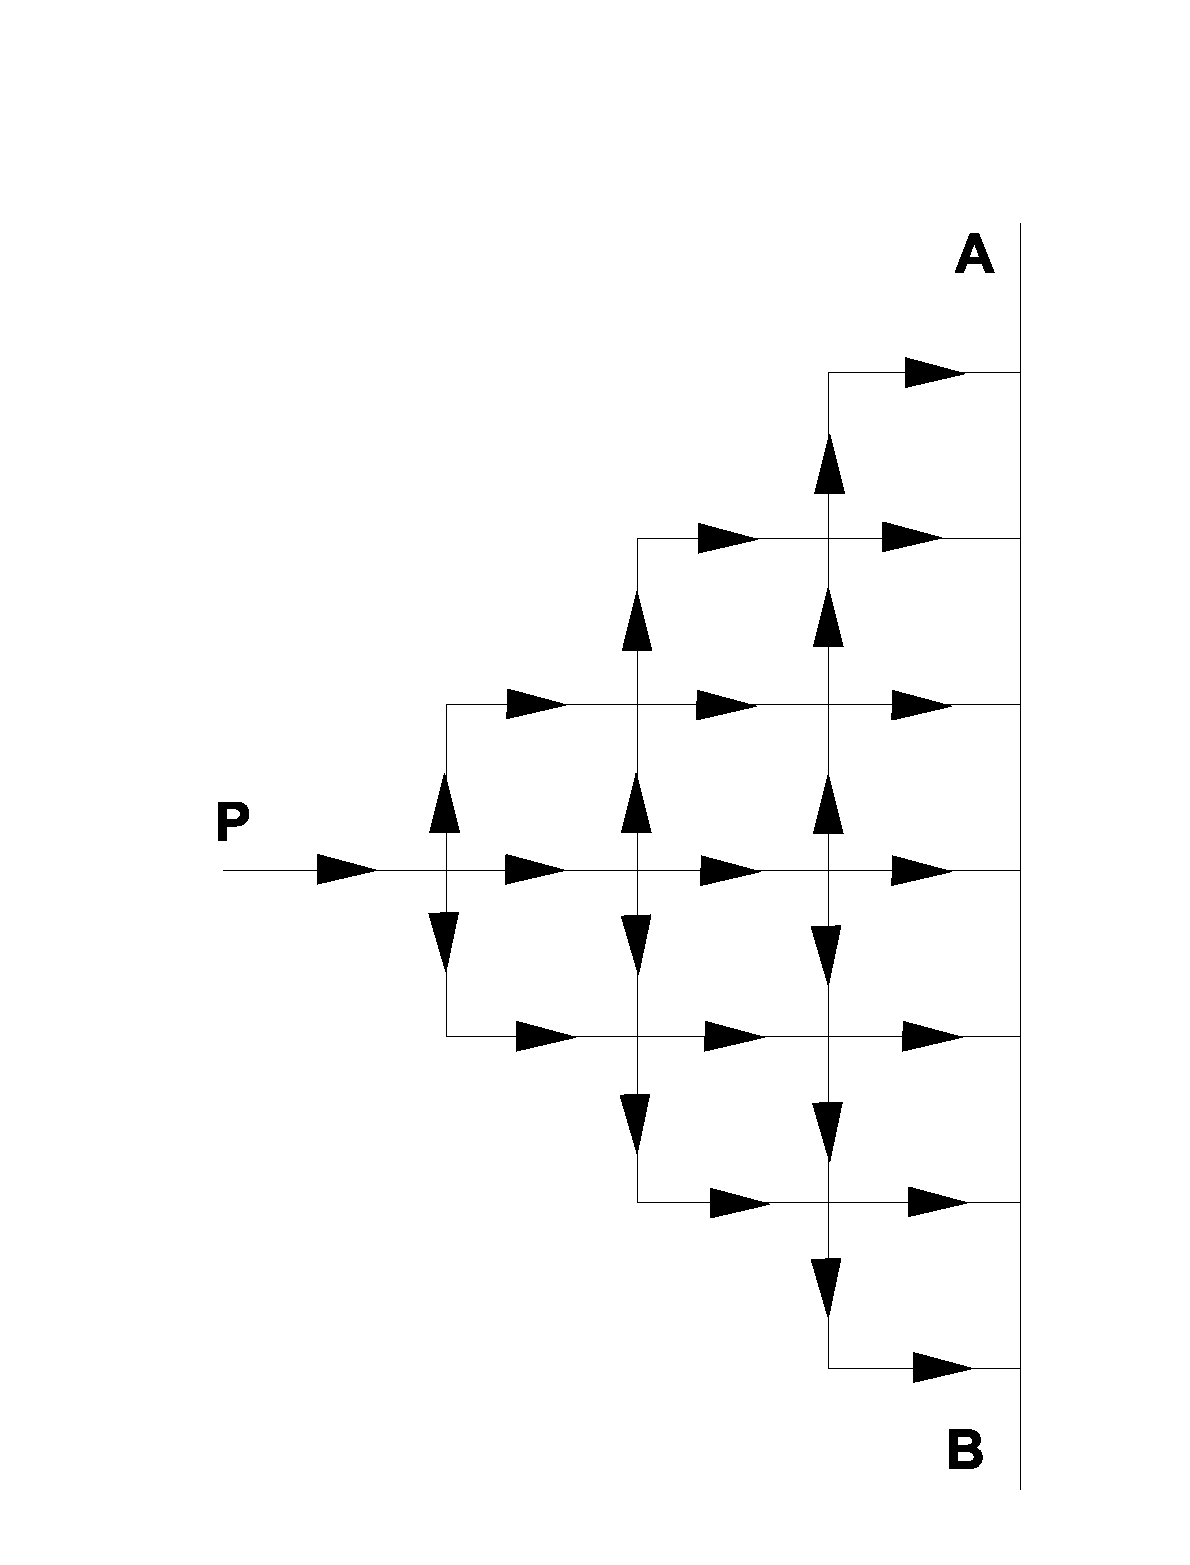
\includegraphics[width=24mm,viewport=86 21 486 641]{CCJPR73-25pic1.eps}
\end{wrapfigure}
On the right we have a map of city streets. All streets, with the exception of AB, are one-way as indicated by the arrows. If a motorist starts at P, how many different routes may he take to reach the two way street AB?\\
%ChoiceA
(A) 81\\
%ChoiceB
(B) 80\\
%ChoiceC
(C) 28\\
%ChoiceD
(D) 27\\
%ChoiceE
(E) 13\\
%Ftext

\begin{wrapfigure}{r}[0pt]{0pt}
	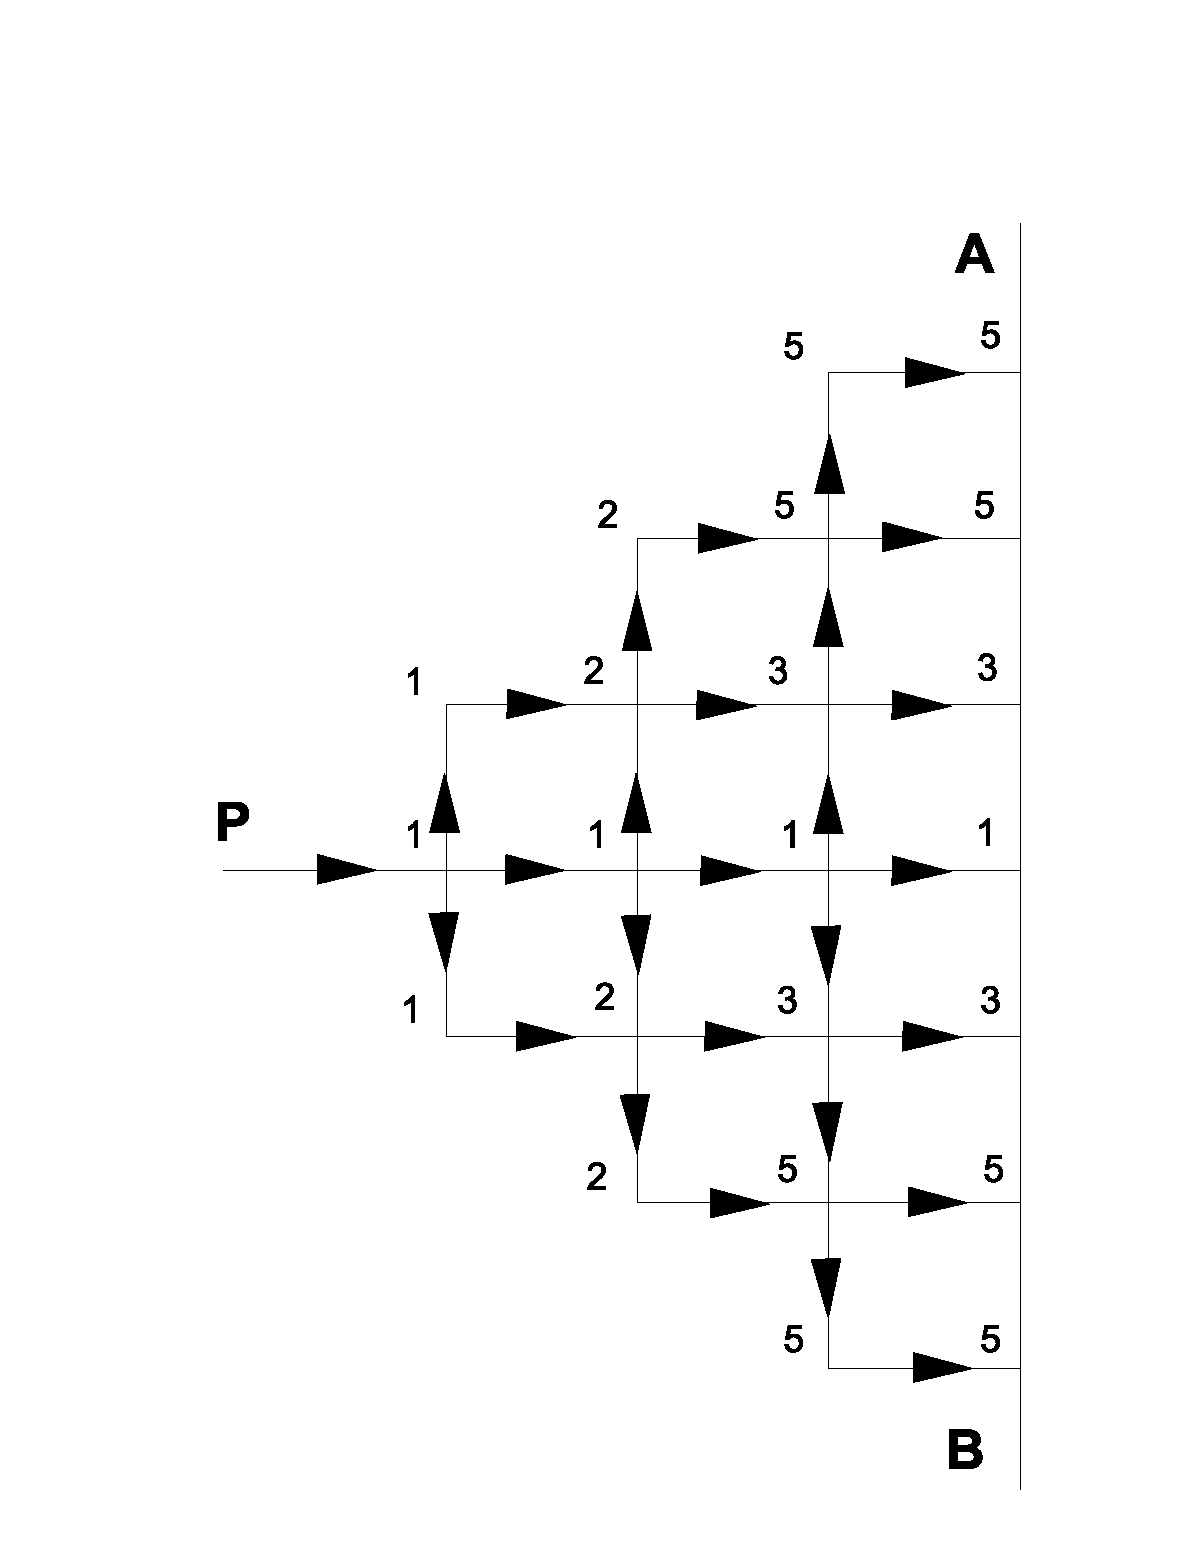
\includegraphics[width=30mm,viewport=89 22 487 642]{CCJPR73-25pic2.eps}
\end{wrapfigure}

\textbf{The correct answer is (D): 27}\\[1 ex]
The figure shows the number of ways to get to each part of the street. If there are 2 ways to reach a street, the traffic on that street could have come from either direction. Thus the number of ways to reach the street is equal to the sum of the ways to reach each street connected to it. Since there are 7 streets connected to street AB, the number of ways to get to it equals the sum of the ways to get to each of the 7 streets.  Thus there are $5+5+3+1+3+5+5=27$ ways.
%End
\end{document}
